\section{本章小结}

本章讨论了不等式,特别讨论了基本不等式和二次函数的最值。

特别要注意四类均值及其关系:
\[
\frac{n}{\sum_{i=i}^n{\frac{1}{x_i}}}\leqslant \sqrt[n]{x_1x_2\cdots x_n}\leqslant \frac{\sum_{i=i}^n{x_i}}{n}\leqslant \sqrt{\frac{\sum_{i=i}^n{x_{i}^{2}}}{n}}
\]
即:
\[
\text{调和}\leqslant \text{几何}\leqslant \text{算数}\leqslant \text{平方}
\]

其次要将基本不等式和二次函数的最值两者融会贯通,通过基本不等式分析二次函数最值的由来。

~

\begin{example}[综合运用5,难度:$\star $]
若$a,b>0$,且$ab=a+b+3$,求$ab$的取值范围。
\end{example}

解一:

题意为求函数$y=ab$的取值范围,且$a,b$有约束$ab=a+b+3$。将约束化简得:
\[
a=\frac{b+3}{b-1} \qquad b>1
\]
带入函数得到:
\[
y=ab=b\cdot \frac{b+3}{b-1} \qquad b>1
\]
不是很明显,但有$x\cdot \frac{1}{x}$的形式,化简该函数:
\begin{align*}
y=b\cdot \frac{b-1+4}{b-1}=\frac{4b}{b-1}+b=\frac{4b-4+4}{b-1}+b=\frac{4}{b-1}+\left( b-1 \right) +5
\end{align*}
易得$\left( b-1 \right) ^2=4$即$b=3$时,$y$有最小值$y_{\min}=9$,函数图象如下。
\begin{figure}[h]
\centering
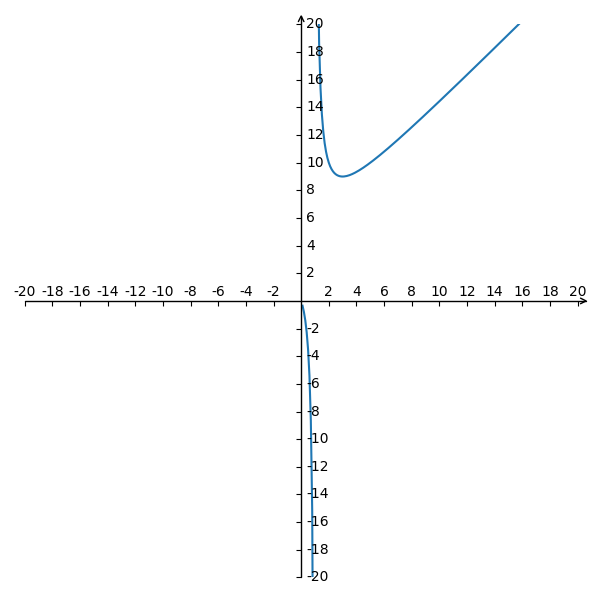
\includegraphics[height=5cm]{2.5-1.png}
\end{figure}

这里,我们将$b\in \left( 0,1 \right) $部分绘制出来,但是由于$a>$的限制,实际$b$的取值范围为$\left( 1,+\infty \right) $。

解二:

观察约束条件和要求的取值函数,$a,b$对称,所以可以直接考察约束条件:
\[
ab=a+b+3\geqslant 2\sqrt{ab}+3
\]
当且仅当$a=b$时成立。于是,可令$y=\sqrt{ab}$,替换得到:
\[
y^2\geqslant y+3 \qquad y>0
\]
易得$y\geqslant 3$,所以当$a=b$时,$ab$取得最小值9。

\begin{tcolorbox}
解一是正经方法,采用了一贯的套路,表达式+约束关系,化简,用基本不等式求解。解二不正经,需要多练,提高洞察力。
\end{tcolorbox}




